\chapter{The tokenized approach}\label{chap:approach}

In the example from the beginning, the problem was that both agents $a$ and $b$ wanted to pull the lever to their own goal which results in infinite executions. This problem can be eliminated by introducing a token. With a token, only the player that has the token gets to execute an action. If the agent is done with their own actions, then they can pass the token on to the next player.

There are different ways to model the token. We are going to start with adding an action that lets one agent hand the token to the next agent. Modeling the token in the beginning of the planning task is a little bit different, since there are three ways the token can be introduced to the agents.
%\todo{Du nimmst bisher keine Referenz zum Kapitel davor. Wuerde das bedeuten, dass man das "Token nehmen" und "Token abgeben" als Aktion in den Planungsalgorithmus einfuehren muss. Dann wuerde ich das hier schreiben.}
\begin{enumerate}
  \item ``Table token'' - the token is lying on a table and one of the agents can take the token in the beginning. \\
  The disadvantage is that maybe no agent would take the token.
  \item ``give token'' - in the specification of the planning task it is also specified which agent will have the token in the beginning. \\
  The problem with this introduction is that in every new planning task, this has to be written in the definition of the task. In order for the planning task to be efficient, it should be given to an agent who has found a plan.
  \item ``random token'' - the token is given to a random agent in the beginning. If that agent can not preform any action it can pass the token to a player who can. \\
  One disadvantage would be that an agent who knows nothing and has no action will prevent the planning task from ever reaching a goal state.
\end{enumerate}

There are also two different types of tokens. The first type of token can be easily passed from one agent to the next without any restriction. This token makes sure that no unwanted agent performs an action that could lead to a worse plan than before. the second type of token forces an agent to perform an action before handing the token to the next agent. This type of token makes sure that the token is not just passed between the agents, it makes sure the agents contribute to reaching a goal state.

\section{Infinite executions to finite executions}

We are now going to describe a function that takes a planning task and tokenize that task. The goal with the tokens is that only one player gets to make a move at a time.

Given a planning task $\Pi = \langle s_0, A, \omega, \gamma \rangle $, the function \textit{tokenize} will transform the planning task into a tokenized planning task so that for all $a \in A$:
 if $a = \langle pre, \textit{eff} \rangle$, then
   $tokenize(a) =\langle pre \wedge hasToken_{\omega(a)}, \textit{eff} \rangle$. \\
Further we define an action
    $ giveToken^{ij} = \langle hasToken_i, \neg hasToken_i \wedge hasToken_j \rangle $
    for all $i,j \in \mathcal{A}$ with $i \not = j$. \\
Then $ A^{Token}=\{tokenize(a)|a \in A\} \cup \{giveToken^{ij}|i,j \in \mathcal{A}, i \not = j\}$. \\
Moreover: $\omega^{Token}(tokenize(a))= \omega(a)$ for all $a \in A$,
and $\omega^{Token}(giveToken^{ij}) = i$ for all $i,j \in \mathcal{A}$. \\
With $s_0$ depending on the way the token should be introduced to the token:

\begin{enumerate}
  \item Table Token:
    The first action in this planning task is for one agent to take the token off the table. Here we need a new action that, if no player has the token, one player can take the token.\\
    $takeToken_j=\langle \bigwedge\limits_{i \in \mathcal{A}}
    \neg hasToken_i, hasToken_j \rangle \forall j \in \mathcal{A}$ with $\omega(takeToken_j)=j$. Then the planning task starts with no agent having the token
    \todo{$s_0 \cup \neg hasToken_i$ macht keinen sinn. Was macht der Mengenvereinigungsoperator auf Zuständen und Propositionen?
* Auch in den anderen Fällen muss die Konstruktion vom neuen $s_0$ noch formal verbessert werden. }
    $s_0^{tableToken} = s_0 \cup \neg hasToken_i$.
    $V_{tableToken}(hasToken_i)=\emptyset \qquad \forall i\in \mathcal{A}$\\
    $V_{tableToken}(p)=V(p) \qquad \forall p\in P : p \not = hasToken$

  \item give Token:
    a specified agent to be determined by the specifications of the planning tasks. We can model this by having $s_0^{giveToken}(j)$ have the variable $j$, the agent that is supposed to have the token in the beginning.
     $s_0^{giveToken}(j) = s_0 \cup \{\neg hasToken_i|i \in \mathcal{A} \backslash j\} \cup hasToken_j$

  \item random Token:
    a random agent
    to model this we need to define some other things first.
    $W_{randomToken}=\{w_i|w \in W, i\in \mathcal{A}\}$ \\
    $w^i \sim_{randomToken} v^i \text{ iff } w \sim v \text{ and } i=j$ \\
    $V_{randomToken}(p)=\{w_i|w\in V(p), p \not = hasToken, i\in \mathcal{A}\}$ \\
    $V(randomToken_i)=\{w_i|w \in W\}$ \\
    $W^{randomToken}_d=\{w_i|w\in W_d, i\in \mathcal{A}\}$ \\
    $s_0^{randomToken}=\langle W_{randomToken}, \sim_{randomToken}, V_{randomToken}, W_{randomToken} \rangle$ \\
    The intuition behind this is duplicating the model for each agent. Because then there are multiple designated worlds, this leads to nondeterminism between the worlds.
\end{enumerate}



Then $ \Pi^{\text{Token}} = \langle s_0^{\text{Token}}, A ^{\text{Token}}, \omega ^{\text{Token}}, \gamma \rangle $.

The action $giveToken$ can have different costs. One option would be to have the the action cost nothing, then the overall cost of the plan would not change. The problem with this is it does not prevent the agents from just passing the token around without a goal. The other option is that the action has the cost 1, then the agents will not just pass the token around,, they will prefer to act themselves if it is more or equally efficient than to let someone else act before handing the token to the next agent.

In searching for the optimal plan the search tree can have a smaller width, because the amount of agents that could perform the next action is limited. Therefore the search tree will probably have a deeper depth, because the action handing off the token will also have to be modeled. This could be researched in the future.

%\extend{Lever example with tokens}

Given this formalization, we can now show that we can stop infinite executions from happening in planning tasks by transforming the planning task into a tokenized planning task.

\begin{theorem}
Under the condition of optimal plans one can prevent the appearance of infinite executions in solvable planning tasks with asynchronous execution order with the introduction of a token based execution order.
\end{theorem}


\begin{proof}[proof sketch]
  The execution is finished when an agent that has the token does not want to do anything. \\
  When an agent $i$ that has a plan gets handed the token, that player has three possible actions:
  \begin{enumerate}
    \item to keep the token and execute an action $a$, which will lower the subjective costs of the remaining policy by at least 1 because the next action is an own action.

    \item to give the token to another agent. In order to pass on the token, the agent that has found the plan would have already performed a perspective shift for the next agent in order to check if the next agent could also find that plan and calculated the subjective cost of the remaining plan. The agent that receives the token will only act with respect to a plan that is at least as good as the plan envisioned by agent $i$.


    \item to do nothing. This will stop the execution.

  \end{enumerate}
  Every agent that will get the token in the plan will either decrease the subjective cost of the policy or stop the execution. Because every agent in the execution decreases the subjective cost, the planning task is executable in infinite executions.
\end{proof}


\section{The prevention of deadlocks}

A deadlock for a policy profile $(\pi_i)_{i \in \mathcal{A}}$ is a global state such that:
\begin{enumerate}
  \item $s$ is not a goal state \\
    Something still needs to be done
  \item $s \in \text{Dom}(\pi_i)$ for some $i \in \mathcal{A}$ \\
    Someone wants something to be done
  \item $\omega(a) \neq i$ for all $i \in \mathcal{A}$ and $a \in \pi_i(s)$ \\
    Nothing will be done because of incompatible individual policies
\end{enumerate}

\begin{wrapfigure}{l}{0.2\linewidth}
\centering
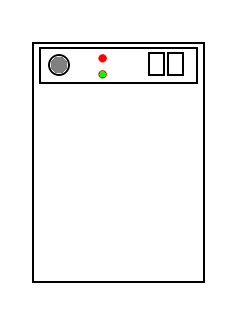
\includegraphics[scale=0.4]{figures/pictures/dishwasher.png}
%\rule{0.9\linewidth}{0.75\linewidth}
%\caption{Dishwasher}
\label{fig:dishwasher}
\end{wrapfigure}


This can be seen in the following example: The two agents from before, Anne and Bill have to empty out the dishwasher. They each have a preference against doing this, since they both spend time (costs) to do this.
In this example you can see that each agent expects the other agent to act, therefore no agent will act.

Let initially, in $s_0$, the dishwasher be full. Agent $1$ has an action $a_1$ and Agent $2$ has an action $a_2$ that can both be applied in $s_0$ and have the effect that has the effect that the dishwasher is empty afterwards. Then the policies $\pi_1 = \{s_0 \xmapsto{a_2} emptyDishwasher \}$ and $\pi_2 = \{s_0 \xmapsto{a_1} emptyDishwasher \}$ are both $i$-strong policies.


Up to this point, the token has given the player that has it the right to perform an action, a right that none of the other players have. But tokens could also force a player to perform an action.

Consider the definition from before with some changes marked in color: \\
Given a planning task $\Pi = \langle s_0, A, \omega, \gamma \rangle $, the function \textit{tokenize-force} will transform the planning task into a tokenized planning task so that for all $a \in A$: \\
 if $a = \langle pre, \textit{eff} \rangle$, then
   $tokenize-force(a) =\langle pre \wedge hasToken_{\omega(a)}, \textit{eff } {\color{UniRed} \wedge doneAction_{\omega(a)}})$ \\
Former we define an Action
    $ giveToken^{ij} = \langle hasToken_i {\color{UniRed}\wedge doneAction_i}, \neg hasToken_i \wedge hasToken_j {\color{UniRed} \wedge \neg doneAction_i} \rangle $
    for all $i,j \in \mathcal{A}$
    \\
Then $ A^{Token}=\{tokenize(a)|a \in A\} \cup \{giveToken^{ij}|i,j \in \mathcal{A}, i \not = j\}
$ \\
Moreover: $\omega^{Token}(tokenize-force(a))= \omega(a)$ for all $a \in A$,
and $\omega^{Token}(giveToken^{ij}) = i$ for all $i,j \in \mathcal{A}$. \\
$s_0^{Token} = s_0 \cup \{\neg hasToken_i|i \in \mathcal{A} \backslash j\} \cup hasToken_j {\color{UniRed} \cup  \{ \neg doneAction_i| i \in \mathcal{A} \}}$ with $j \in \mathcal{A}, |j|=1$\\

With $s_0$ depending on the way the token should be introduced to the token:
\begin{enumerate}
  \item Table Token: The first action in this planning task is for one agent to take the token off the table. Here we need a new action that, if no player has the token, one player can take the token.\\
    $takeToken_j=\langle \bigwedge\limits_{i \in \mathcal{A}}
    \neg hasToken_i, hasToken_j \rangle \forall j \in \mathcal{A}$ with $\omega(takeToken_j)=j$. \\
    Then the planning task starts with no agent having the token or having done an action \\
    $s_0^{tableToken} = s_0 \cup \neg hasToken_i \cup \neg doneAction_i$ \\
    $V_{tableToken}(hasToken_i)=\emptyset \text{ and } V_{tableToken}(doneAction_i)=\emptyset \qquad \forall i\in \mathcal{A}$\\
    $V_{tableToken}(p)=V(p) \qquad \forall p\in P : p \not = hasToken, doneAction$

  \item give Token:
    a specified agent to be determined by the specifications of the planning tasks. We can model this by having $s_0^{giveToken}(j)$ have the variable $j$, the agent that is supposed to have the token in the beginning. \\
     $s_0^{giveToken}(j) = s_0 \cup \{\neg hasToken_i|i \in \mathcal{A} \backslash j\} \cup hasToken_j \cup \{\neg doneAction_i|i \in \mathcal{A}\}$

  \item random Token:
    a random agent
    to model this we need to define some other things first.
    $W_{randomToken}=\{w_i|w \in W, i\in \mathcal{A}\}$ \\
    $w^i \sim_{randomToken} v^i \text{ iff } w \sim v \text{ and } i=j$ \\
    $V_{randomToken}(p)=\{w_i|w\in V(p), p \not = hasToken, i\in \mathcal{A}\}$ \\
    $V(randomToken_i)=\{w_i|w \in W\}$ \\
    $W^{randomToken}_d=\{w_i|w\in W_d, i\in \mathcal{A}\}$ \\
    $s_0^{randomToken}=\langle W_{randomToken}, \sim_{randomToken}, V_{randomToken}, W^{randomToken}_d \rangle$ \\
    \todo{Wie modelliere ich hier doneAction rein?}
    The intuition behind this is duplicating the model for each agent. Because then there are multiple designated worlds, this leads to nondeterminism between the worlds.
\end{enumerate}



Then $ \Pi^{\text{Token}} = \langle s_0^{\text{Token}}, A ^{\text{Token}}, \omega ^{\text{Token}}, \gamma \rangle $.

The changes imply that each agent can only pass on the token when that agent has performed an action.

This new token version also solves the infinite execution problem.

The table token introduction of the token does not prevent deadlocks because in this case, no agent would take the token off the table, which causes a deadlock. Also, the deadlock in this case can only appear in the initial state, in every other state there is always exactly one acting agent.
\todo{Ist das so verständlich?}

\begin{theorem}
  Under the condition of optimal plans one can prevent the appearance of infinite executions in solvable planning tasks with asynchronous execution order with the introduction of a force token based execution order.
\end{theorem}



\begin{proof}[proof sketch]
  The execution is finished when an agent that has the token does not want to do anything. \\
  When an agent $i$ that has a plan gets handed the token, that player first has to perform an action, thereby lowering the subjective cost, and then that player has two possible actions:
  \begin{enumerate}
    \item to keep the token and execute another action, which will lower the subjective costs of the remaining policy profile or
    \item to give the token to another agent. In order to pass on the token, the agent that has found the plan would have already performed a perspective shift for the next agent in order to check if the next agent could also find that plan and calculated the subjective cost of the remaining plan. The agent that receives the token will only act with respect to a plan that is at least as good as the plan envisioned by agent $i$.
  \end{enumerate}
  Every agent that will get the token in the plan will either decrease the subjective cost of the policy or stop the execution. Because every agent in the execution decreases the subjective cost, the planning task is executable in infinite executions.
\end{proof}

\begin{theorem}
Under the condition of optimal plans one can prevent the appearance of deadlocks in planning tasks with asynchronous execution order with the introduction of a force token based execution order with the give token and random token introduction of the token.
\end{theorem}

\begin{proof}[proof sketch]
  Before any player can give away the token, that player has to perform an action. If a player that has found a plan gets the token, that agent first has to do an action. This contradicts the definition of a deadlock.
\end{proof}


\begin{theorem}
  Under the condition of optimal plans one can prevent the appearance of deadlocks in solvable games with asynchronous execution order with the introduction of a token based execution order with the exception of the table token introduction of the token, as long as the giveToken action costs at least 1.
\end{theorem}

\begin{proof}[proof sketch]
  In every agents policy there is an exact sequence of acting agents. Because only one agent can act, the state that some agents are waiting on each other will never appear.
  The one acting agent will then specify the next acting agent, therefore there always will be something done.
\end{proof}


With these results, we do not need to enforce the agents to be eager to avoid deadlock if we use the tokens with costs. We also do not need optimally eager agents to prevent infinite executions if we use tokens. The only problem with tokens is the introduction of the token, especially with the table token. But as long as an agent takes the token off the table, there will be no more deadlocks.
